\documentclass[11pt,letterpaper]{article}
\usepackage[utf8]{inputenc}
\usepackage[spanish,es-nodecimaldot]{babel}
\usepackage{amsmath}
\usepackage{amsfonts}
\usepackage{amssymb}
\usepackage{color,soul}
\usepackage{textcomp}
\usepackage{stmaryrd}
\usepackage{makeidx}
\usepackage{colortbl}
\usepackage{tocloft}
\renewcommand{\cftsecleader}{\cftdotfill{\cftdotsep}}
\usepackage{rotating}
\usepackage{url}
\usepackage{pdflscape} 
\usepackage{pdfpages}
\usepackage{float}
\usepackage{graphicx}
\usepackage{ marvosym }
\usepackage{pgf,tikz}
\usepackage{mathrsfs}
\usetikzlibrary{arrows}
\usepackage{ mathrsfs }
 \usepackage{array}
\usepackage{longtable}
\newcommand{\justif}[2]{&{#1}&\text{#2}}
\usepackage{listings}
\usepackage{color}
\newcolumntype{L}[1]{>{\raggedright\let\newline\\\arraybackslash\hspace{0pt}}m{#1}}
\newcolumntype{C}[1]{>{\centering\let\newline\\\arraybackslash\hspace{0pt}}m{#1}}
\newcolumntype{R}[1]{>{\raggedleft\let\newline\\\arraybackslash\hspace{0pt}}m{#1}}
\definecolor{dkgreen}{rgb}{0,0.6,0}
\definecolor{gray}{rgb}{0.5,0.5,0.5}
\definecolor{mauve}{rgb}{0.58,0,0.82}
\setboolean{@twoside}{false}
\lstset{frame=tb,
  language=Java,
  aboveskip=3mm,
  belowskip=3mm,
  showstringspaces=false,
  columns=flexible,
  basicstyle={\small\ttfamily},
  numbers=left,
  numberstyle=\tiny\color{gray},
  keywordstyle=\color{blue},
  commentstyle=\color{dkgreen},
  stringstyle=\color{mauve},
  breaklines=true,
  breakatwhitespace=true,
  tabsize=3
}

\usetikzlibrary{graphs,graphs.standard}
\newcommand{\floor}[1]{\lfloor #1 \rfloor}

\usepackage{multicol}

\usepackage{caption}
\usepackage{subcaption}
\begin{document}
\begin{titlepage}
	\centering
	{\scshape\LARGE Universidad Nacional Autónoma de México \par}
	\vspace{1cm}
	{\scshape\Large Facultad de Ciencias\par}
	\vspace{1.5cm}
\begin{center}
		
\includegraphics[scale=.5]{logo.png}
	\end{center}
		\vspace{.8 cm}

	{\huge\bfseries Proyecto Final: \par}
	{\huge\bfseries Diagrama Entidad-Relación \par}
		\vspace{0.5cm}

	{\Large\itshape Flores Martínez Andrés\\
	Vázquez Salcedo Eduardo Eder\\
	Sánchez Pérez Pedro Juan Salvador\\
	Concha Vázquez Miguel\par}
	\vfill
			\vspace{0.5cm}

	Trabajo presentado en cumplimiento con la asignatura de Fundamentos de Bases de Datos impartida por el profesor	\par
	 \textsc{Gerardo Avilés Rosas}\\
	\vspace{0.1cm}
	{\large 12 de enero de 2018\par}
\end{titlepage}



\newpage





\begin{landscape}

\begin{center}
\begin{minipage}{.8\linewidth}
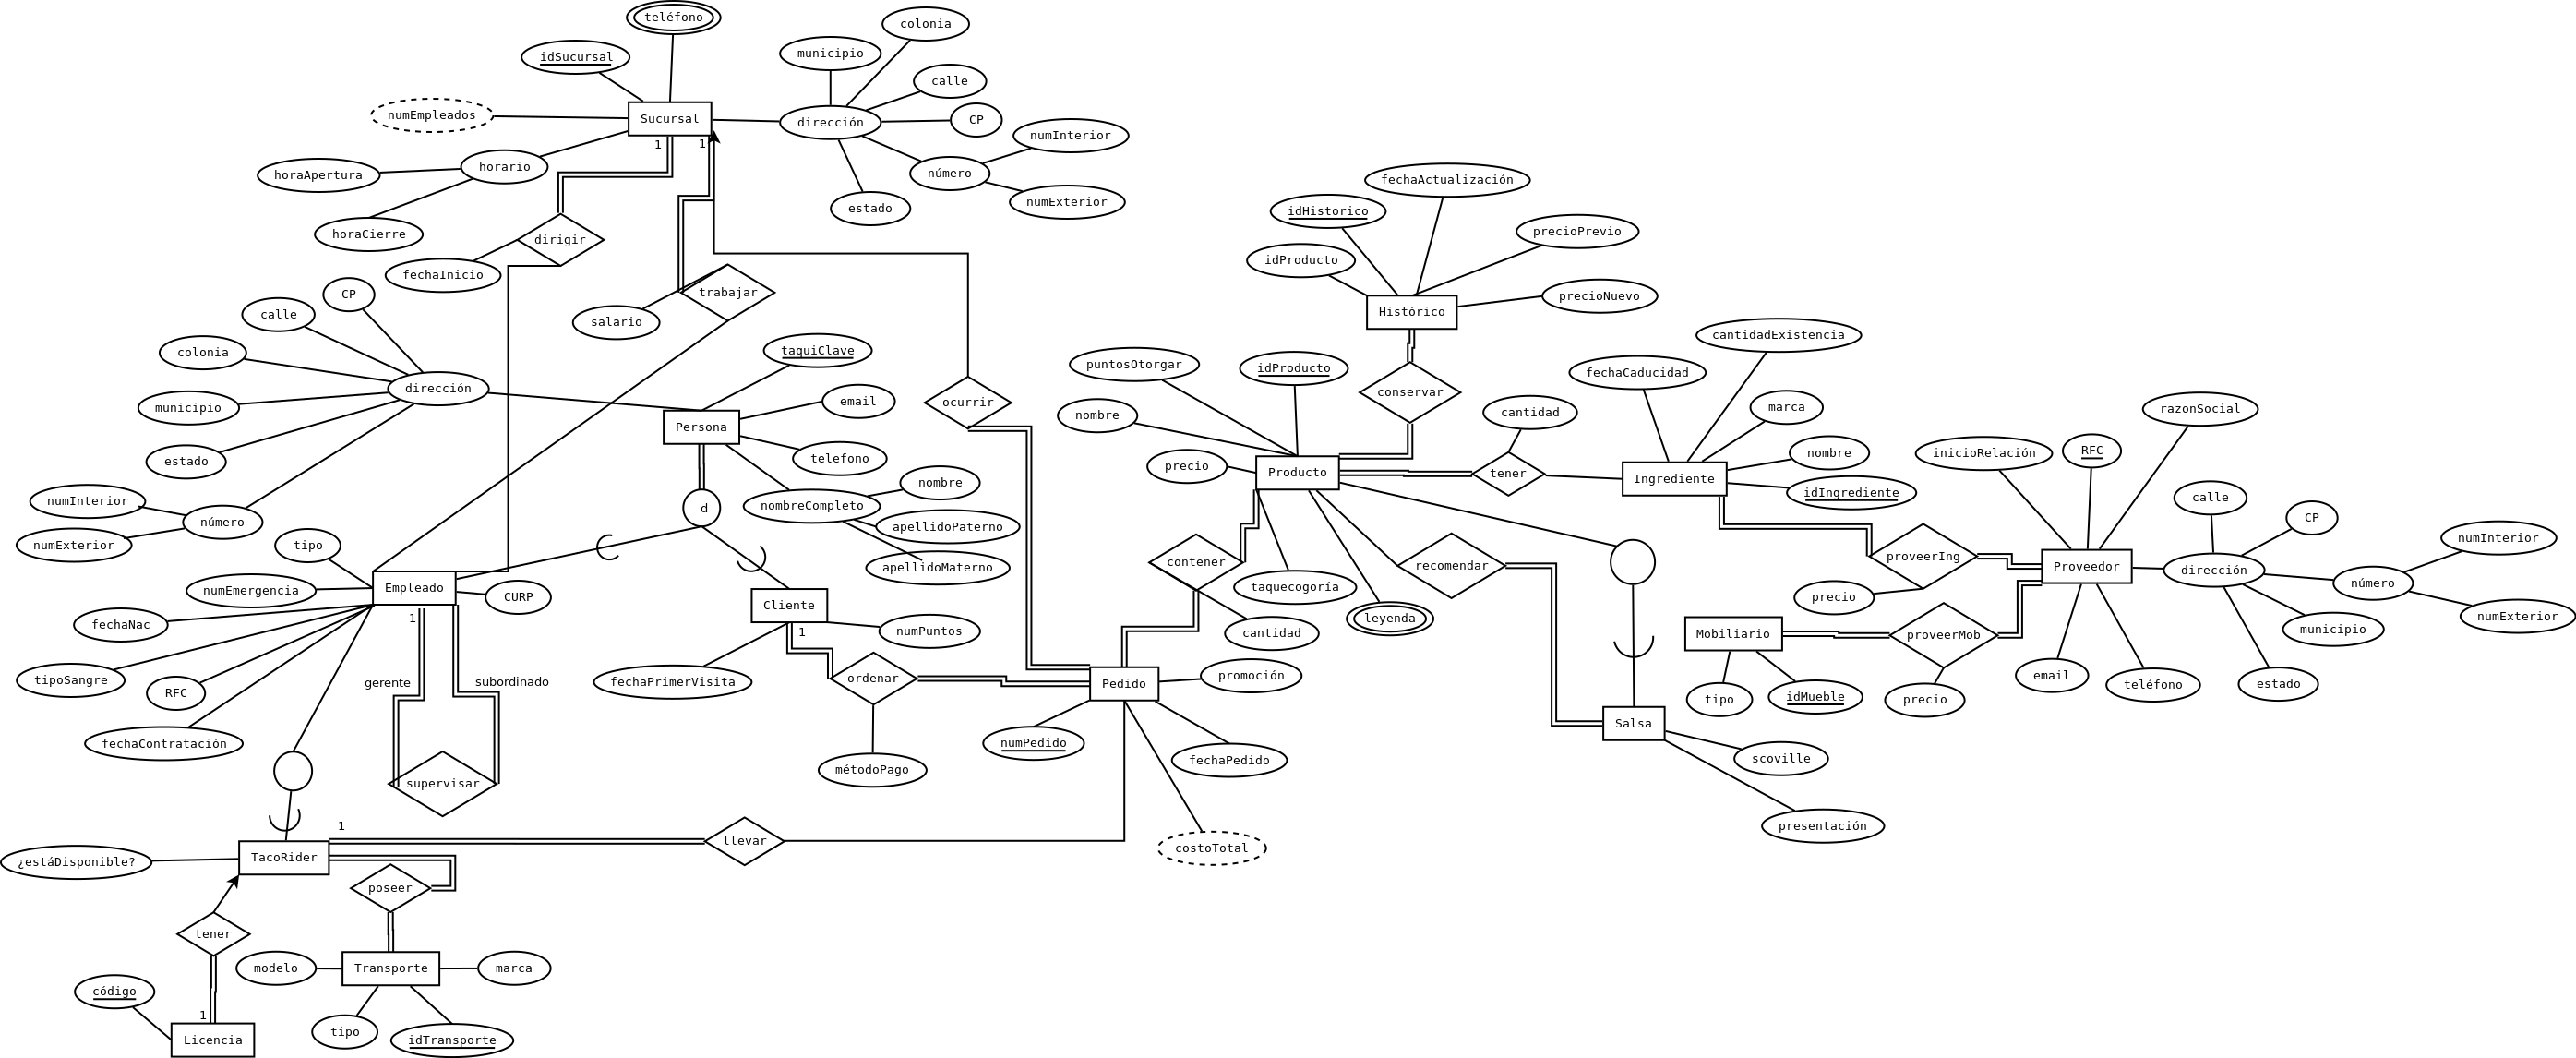
\includegraphics[scale=0.22]{ER.png}
\captionof{figure}{Diagrama Entidad-Relación (formalismo de diseño) resultante del modelado a partir del caso de uso y el documento de análisis de requerimientos.}
\end{minipage}
\end{center}

\end{landscape}


\newpage
\textbf{A continuación detallaremos nuestras elecciones para la construcción del diagrama entidad-relación (E/R) del caso de uso de la taquería \textit{Tacoste} planteado a partir de nuestro documento de análisis de requerimientos:}\\


Lo primero que hicimos fue seguir la recomendación de identificar en primera instancia a las entidades principales involucradas en el caso de uso, a pesar de que sabíamos que probablemente iban a irse viendo modificadas en
el proceso. Evidentemente ---a partir del documento de análisis de requerimientos--- era importante considerar como entidades fuertes a los \textit{clientes} de las distintas \textit{sucursales} de las taquerías, así como también a los empleados que laboran en las mismas. \\

Sin embargo, desde un inicio notamos que había propiedades particulares que eran compartidas tanto por los clientes como por los empleados; estos atributos entonces fueron abstraídos en una super-entidad \textbf{Persona} y fueron: \textit{email} (dirección de correo electrónico)\footnote{Consideramos que es suficiente contar con una sola dirección de correo por cada persona.}, \textit{teléfono} (número telefónico)\footnote{Asimismo, suponemos que basta con tomar en cuenta un único número telefónico por cada persona.} y el \textit{nombreCompleto}, siendo este último un atributo compuesto conformado por el \textit{nombre}, \textit{apellidoPaterno} y el \textit{apellidoMaterno} del individuo. También añadimos un atributo compuesto con los datos de la \textit{dirección} de la persona, constituido este último por los atributos del \textit{CP} (código postal),  \textit{calle}, \textit{colonia}, \textit{municipio}, \textit{estado} y \textit{número}\footnote{Decidimos que había que definir al atributo \textit{número} como un atributo compuesto que incluyera un \textit{numInterior} y \textit{numExterior} para ser más precisos.}. Como identificador incluimos una llave subrogada incremental que sería común a todo individuo que tuviera relación con las taquerías y que llamamos \textit{taquiClave}.\\

Luego, aprovechando las capacidades ofrecidas por el modelo E/R extendido (EER), fue posible a través de la especialización definir dos sub-entidades que tuvieran asociados los atributos de \textbf{Persona} y que diera cabida también a establecer relaciones específicas adicionales entre las sub-entidades y otras que definiríamos más adelante; estas sub-entidades fueron justamente las de \textbf{Empleado} y \textbf{Cliente}.\\

\newpage 
En la especialización definimos una restricción de disyunción para poder establecer que bajo nuestro esquema no era posible que un empleado fuera a su vez un cliente de la taquería\footnote{Dado el caso en que un posible empleado quisiera ir, por ejemplo, a comer el fin de semana con su familia a alguna sucursal, entonces sería todavía considerado como un empleado para evitar la duplicidad de la información en la base de datos. Esta posibilidad tiene cabida dentro del modelo planteado puesto que las relaciones de \textit{pedidos} y demás ocupan el identificador de la \textbf{Persona}: la \textit{taquiClave} que es común tanto a personas como a empleados.}. Subsecuentemente establecimos también una restricción de completez de especialización total, pues forzosamente ocurría que todo individuo del cual íbamos a almacenar información era forzosamente un cliente o un empleado de la taquería.\\


En particular, para la sub-entidad \textbf{Empleado} agregamos como sus atributos el \textit{CURP}, \textit{RFC}, \textit{tipo} (referente al tipo de empleado en cuestión), \textit{tipoSangre}, \textit{fechaNac} (fecha de nacimiento)\footnote{A partir de esta información podríamos posteriormente obtener la edad de cada empleado.}, \textit{numEmergencia} (un número telefónico de alguna persona de contacto en caso de algún percance o emergencia) y la fecha de contratación del empleado para poder tener información de su antigüedad al que llamamos \textit{fechaContratación}. 
En cuanto al conjunto entidad \textbf{Cliente}, incluimos como sus atributos \textit{numPuntos} para poder determinar el número de puntos acumulados por cada cliente bajo el programa de \textbf{taquero mucho} y un atributo \textit{fechaPrimerVisita} para poder determinar la primera vez que consumió en alguna sucursal; esto nos podría servir para poder ---en algún momento--- dar beneficios a los clientes más antiguos.\\

Para la entidad fuerte \textbf{Sucursal} que identificamos a partir del análisis de requerimientos, incluimos como sus atributos un identificador \textit{idSucursal} que funcionaría como su llave primaria, un atributo compuesto \textit{horario} que incluía a su vez la \textit{horaApertura} y \textit{horaCierre} de las sucursales, el atributo compuesto \textit{dirección} que de nueva cuenta estaba conformado por \textit{municipio}, \textit{colonia}, \textit{calle}, \textit{CP}, \textit{estado} y el atributo a su vez compuesto de \textit{numInterior} y \textit{numExterior} de \textit{número}. Como pensamos que era importante prever la posibilidad de que una misma sucursal tuviera varios teléfonos de contacto, entonces agregamos un atributo multivaluado \textit{teléfono} y también un atributo calculado de \textit{numEmpleados} para poder conocer cuántos empleados laboran en cada sucursal de Tacoste.\\

\newpage
A partir de las entidades definidas hasta el momento fue posible definir dos relaciones entre la sub-entidad \textbf{Empleado} y la entidad \textbf{Sucursal} a partir del papel que cada una desempaña. Era importante conocer al gerente de cada sucursal a pesar de que no estaba especificado en el caso de uso, pero sí en nuestro análisis de requerimientos con tal de tener escalabilidad. Así, establecimos una relación \textit{dirigir} entre las entidades previamente mencionadas, con un atributo de relación \textit{fechaInicio} para poder llevar cuenta del tiempo en que el gerente ha desempeñado su papel. \\

Para esta relación binaria, la restricción de participación fue parcial del lado de \textbf{Empleado} teniendo en cuenta que no todos los empleados forzosamente eran gerentes, y fue total del lado de \textbf{Sucursal}, pues no pueden haber sucursales sin supervisores. Para la restricción de cardinalidad, la definimos de tipo muchos-uno ya que un empleado puede solamente estar asociado a una sucursal, no dando así cabida a que un gerente sea dirigente de varias sucursales a la vez; por otro lado, una misma sucursal consideramos que puede tener más de un gerente ya que puede ser que estén enfocados a dirigir áreas ajenas.\\

La segunda relación establecida entre \textbf{Sucursal} y \textbf{Empleado} fue la de \textit{trabajar}, identificada a partir del análisis de requerimientos y evidente desde el caso de uso. Entonces, para poder identificar el salario de cada empleado, nos pareció oportuno incluir un atributo de relación \textit{salario}. La restricción de participación fue parcial del lado del empleado en el sentido en que podrían haber personas como  el señor Pepe que no necesariamente laboraran en una sucursal en el sentido de que llevan un control más global de la taquería; del lado de Sucursal fue total para indicar que no puede haber sucursales sin empleados. Para la restricción de cardinalidad, impusimos un esquema muchos-uno para indicar que los empleados pueden estar asociados a una única sucursal como indicamos en las restricciones solicitadas, pero que en una sucursal puede laborar más de un empleado. \\

También notamos que era necesario poder identificar a los jefes particulares de cada empleado, estableciendo así una nueva relación binaria de la entidad \textbf{Empleado} consigo misma que definimos con el nombre \textit{supervisar}. A pesar de que no era obligatorio, decidimos etiquetar los roles de participación de ambas partes con ``gerente"\,\, y ``subordinado", teniendo así una mayor claridad. La participación fue total de ambos lados, pues no puede haber empleados sin algún tipo de jefe, como tampoco jefes sin subordinados. Además, la restricción de cardinalidad fue de tipo uno-muchos, pues un mismo gerente puede tener a varios empleados bajo su supervisión, pero cada empleado puede tener un solo empleado al cual responde directamente.\\

A pesar de que ya habíamos considerado un atributo para el tipo de empleado en el conjunto entidad de \textbf{Empleado} que nos permitiría definir a los parrilleros, meseros, taqueros, cajeros, tortilleros, repartidores y dando cabida a la escalabilidad, decidimos finalmente abstraer a los repartidores en una sub-entidad de los empleados que llamamos \textbf{TacoRider}. La razón principal fue la de poder almacenar información adicional de éstos últimos a raíz de los datos que tendrían que tener de los pedidos a domicilio, su licencia (cuando aplicara) y los datos de los vehículos utilizados por ellos. La restricción de completez en esta especialización fue parcial, pues no todo empleado es necesariamente un repartidor. No fue necesario establecer ninguna restricción de disyunción al tratarse de una única sub-entidad. Como atributo incluimos uno de tipo booleano que llamamos \textit{¿estáDisponible?} para poder saber si está en condición de hacer un envío en un momento determinado. \\

Al ser la licencia algo opcional y que aplica en ocasiones dependiendo del tipo de vehículo utilizado por el repartidor, decidimos crear una nueva entidad fuerte \textbf{Licencia}. A primera vista pensamos que se trataba de una entidad débil forzosamente debía existir un repartidor para poder existir un registro de la licencia. No obstante, luego caímos en cuenta de que en emergencias sería posible hacer que algún otro empleado de otro tipo se convirtiera momentáneamente en \textbf{tacoRider} con tal de hacer entregas a domicilio. Bajo esta lógica, las licencias podrían existir aún cuando todavía no estuviera contemplado un empleado particular como un repartidor para poder decidir justamente quién era candidato a realizar una entrega en motocicleta. El único atributo que incluimos en la entidad \textbf{Licencia} fue el de su \textit{código}, mismo que funge como llave de la entidad fuerte.\\

La relación binaria creada entre la \textbf{Licencia} y el \textbf{TacoRider} fue la de \textit{tener}. La restricción de participación fue total del lado de la \textbf{Licencia} y parcial del lado de \textbf{TacoRider} para contemplar la posibilidad de que no tuviera una licencia al moverse únicamente en bicileta como se especificaba en el documento de análisis de requerimientos. La restricción de cardinalidad fue de uno-uno porque un repartidor no puede tener más de una licencia legalmente, así como una licencia no puede pertenecer a más de un repartidor.\\

\newpage 
De igual manera identificamos una nueva relación \textit{poseer} entre las dos entidades previamente descritas para poder tomar en cuenta a los medios de transporte. Así, también fue necesario crear una entidad \textbf{Transporte}. Decidimos que la entidad era fuerte en el sentido en que los transportes podrían existir inclusive cuando no hubiera repartidores porque serían de la taquería propiamente. Para dicha entidad consideramos como atributos una llave subrogada \textit{idTransporte}, \textit{marca}, \textit{modelo} y \textit{tipo}. Poder presentar el tipo del vehículo de esta manera ofrece escalabilidad ya que eventualmente los dueños de la taquería pueden plantearse la inclusión de vehículos de entrega de nuevo tipo, como automóviles. \\

En cuanto a la relación \textit{poseer}, la restricción de participación fue total de ambos lados para indicar que todo repartidor debe tener un vehículo asignado, y todo vehículo debe ser usado por algún repartidor, pues sería un desperdicio para la taquería comparar vehículos sobrantes y desde el caso de uso se busca una optimización de recursos monetarios. Luego, la restricción de cardinalidad fue de muchos-muchos para indicar que un mismo vehículo peude ser eventualmente conducido por distintos repartidores, y que un mismo repartidor puede utilizar distintos medios de transporte para la entrega de los pedidos. \\

Como siguiente paso en el proceso del diseño del diagrama, comenzamos a definir entidades fuertes para \textbf{Pedido}, \textbf{Producto}, \textbf{Salsa} e  \textbf{Ingrediente} como habíamos podido observar a través de lo definido en el análisis de requerimientos. \\

En lo que respecta a los productos vendidos en las taquerías Tacoste, decidimos incluir como atributos una llave primaria \textit{idProducto}, el \textit{nombre}, su \textit{precio} y el número de puntos que genera el producto para poder asegurar escalabilidad en el sentido en como la empresa maneja el proyecto de \textit{taquero mucho}. También consideramos la \textit{taquegoría} de cada producto (categoría) y un atributo multivaluado para las \textit{leyendas} que puede tener el producto y que se presentan en el menú como pueden ser light, vegano, orgánico, etcétera.\\

Para los ingredientes, de forma similar añadimos como atributos una llave \textit{idIngrediente}, \textit{nombre}, \textit{marca}, \textit{fechaCaducidad} (con tal de evitar potenciales desperdicios), y la \textit{cantidadExistencia} para poder darse cuenta del momento en que resulta necesario la compra de más ingredientes de cierto tipo. \\

Para la entidad \textbf{Salsa}, notamos que tenía que tener los atributos de \textbf{Producto}, además de \textit{presentación}, y \textit{scoville} para contemplar el nivel de picor de cada salsa. Por ende, impusimos un esquema de especialización, considerando a la \textbf{Salsa} como sub-entidad de \textbf{Producto}. No hubo necesidad de imponer restricciones de disyunción al ser solamente un conjunto de entidades especializado; para la restricción de completez, la especificamos parcial ya que no todo producto es necesariamente una salsa.\\

Ahora, para la entidad fuerte de \textbf{Pedido} definimos como atributo llave el \textit{numPedido}, pero también consideramos como atributos la \textit{fechaPedido}, \textit{promoción}\footnote{Estamos evitando a toda costa los valores nulos en nuestro diseño, por lo que en caso de que no aplique alguna promoción, tendremos que especificarlo explícitamente en la base de datos.}, así como un atributo calculado de \textit{costoTotal}. \\

A partir de estas nuevas entidades fuertes definimos nuevas relaciones. Como los repartidores se encargan de entregar pedidos a domicilio, entonces creamos una relación con restricción de cardinalidad uno-mucho llamada \textbf{llevar} entre \textbf{TacoRider} y \textbf{Pedido}. El motivo fue que cada pedido es entregado por un solo repartidor, pero un mismo repartidor puede hacer entrega de múltiples pedidos. Ahora, para la restricción de participación se especificó como total del lado de \textbf{TacoRider} porque no puede haber repartidores que no hagan entregas; fue parcial del lado de \textbf{Pedido} ya que puede haber órdenes que tienen lugar dentro de las sucursales físicamente, así que no se tiene que hacer un envío a domicilio.\\

Se especificó también una relación \textit{ordenar} con restricción de cardinalidad uno-muchos entre \textbf{Cliente} y \textbf{Pedido}, pues un mismo cliente puede hacer múltiples pedidos, pero no puede ocurrir que un mismo pedido corresponda a más de un cliente. De esta forma solucionamos el inconveniente de las mesas, pues estamos definiendo que cada pedido estará asociado en estos escenarios con algún cliente de dicha mesa que actúa como responsable de la compra. Como atributo de la relación incluimos \textit{métodoPago} para especificar la forma en la que se efectuó el cobro del pedido (tarjeta de crédito o débito, efectivo, vales, cripto-moneda, etcétera). Finalmente, la restricción de participación fue total de ambos lados, pues forzosamente un cliente de la taquería efectúa pedidos por definición de cliente, así como los pedidos tiene que ser hechos por clientes.\\

Como se llevan a cabo los pedidos en las sucursales, establecimos una relación \textit{ocurrir} entre \textbf{Sucursal} y \textbf{Pedido}. La restricción de cardinalidad fue de uno-muchos, pues en una sucursal se pueden presentar varios pedidos, pero un pedido no puede tener lugar en más de una sucursal. Fue total del lado de \textbf{Pedido}, pues forzosamente tiene que ocurrir en una sucursal para poder definirse; en cuando a \textbf{Sucursal}, su participación es parcial, pues puede haber sucursales registradas que todavía no hayan registrado ningún pedido. \\

Luego, definimos una relación binaria de nombre \textit{contener} entre los conjuntos de entidades  fuertes \textbf{Producto} y \textbf{Pedido} con atributo de relación \textit{cantidad} para poder registrar la cantidad de cada producto por pedido. La restricción de participación fue total de ambos lados, pues un pedido forzosamente tiene productos y un los productos necesariamente forman parte de algún pedido. Más aún, la restricción de cardinalidad la definimos de tipo muchos-muchos, pues un pedido puede consistir de más de un producto, así como un producto puede estar presente en varios pedidos.\\

La relación con nombre \textit{tener} que definimos entre \textbf{Producto} e \textbf{Ingrediente} fue a raíz de nuestro documento de análisis de requerimientos y su restricción de cardinalidad de tipo muchos-muchos. Esto último se debió a que un ingrediente puede estar presente en varios productos, así como un producto puede llevar más de un ingrediente ---y generalmente este es el caso. Ahora, la restricción de participación fue total del lado de \textbf{Producto} porque forzosamente se componen de ingredientes y parcial del otro lado, pues podemos tener ingredientes en una sucursal que todavía no hayan sido usados y en consiguiente no formen parte de algún producto. También añadimos un atributo de relación \textit{cantidad} para poder justamente indicar la fracción del ingrediente presente en cada producto.\\

Dado que de acuerdo al caso de uso y a lo reflejado por el análisis de requerimientos en la sección de relaciones entre los datos era necesarios que las salsas recomendaron productos con qué acompañarlas, entonces definimos una relación \textit{recomendar} entre \textbf{Producto} y \textbf{Salsa}. La restricción de participación fue parcial del lado de \textbf{Producto}, pues los productos no necesariamente recomiendan salsas; lo contrario no puede decirse, pues necesariamente ocurre y entonces fue total del lado del conjunto entidad \textbf{Salsa}. La restricción de cardinalidad fue muchos-muchos para contemplar la posibilidad de que un producto pueda recomendar muchas salsas y viceversa. \\

El siguiente paso en la creación del diagrama fue el establecimiento de una nueva entidad fuerte para los proveedores: \textbf{Proveedor}. Para poder hacer la diferenciación entre el tipo de bienes que proveen, creamos una entidad \textbf{Mobiliario} con atributos \textit{tipo} y un \textit{idMueble} como una llave. En cuanto a los proveedores, agregamos atributos de \textit{inicioRelación}\footnote{El motivo de esto fue para considerar la fiabilidad de cada proveedor a partir de la antigüedad de la relación para considerar la realización de alianzas comerciales como se había especificado en el caso de uso.}, \textit{RFC} como llave, \textit{razónSocial}, teléfono, \textit{email}\footnote{Así como con las personas, consideramos suficiente almacenar un registro de un único número telefónico y dirección de correo electrónico como forma de contacto para cada proveedor.} y el atributo compuesto correspondiente a la \textit{dirección}: \textit{CP}, \textit{colonia}, \textit{calle}, \textit{municipio}, \textit{estado} y el atributo compuesto de \textit{numInterior} y \textit{numExterior} del \textit{número}.\\

Como siguiente paso, establecimos dos relaciones análogas con atributo \textit{precio} entre la entidad \textbf{Proveedor} y las entidades respecivas de \textbf{Ingrediente} y \textbf{Mobiliario}. Las restricciones en ambos casos fueron las mismas: en cuando a la participación fue total de ambos lados y de cardinalidad muchos-muchos. Las razones fueron que forzosamente los proveedores tienen que hacer entrega de dichos bienes (según sea el caso) y estos bienes tienen que ser necesariamente entregados por los proveedores con tal de no romper potenciales alianzas comerciales. Además, un mismo proveedor puede hacer entrega de varios bienes, y un mismo bien puede ser provisto por distintos proveedores. A dichas relaciones las llamamos \textit{proveerIng} en el caso de la relación binaria entre \textbf{Proveedor} e \textbf{Ingrediente}; para la relación binaria entre \textbf{Proveedor} y \textbf{Mobiliario} la llamamos \textit{proveerMob}.\\

La última fase de traducción consistió en considerar a la entidad fuerte \textbf{Histórico} ya identificada en el análisis de requerimientos. Dicha entidad tenía como atributos el \textit{idProducto}, \textit{fechaActualización}, \textit{precioPrevio} y \textit{precioNuevo} tras la actualización. El identificador del producto funcionó como atributo llave de la entidad. Establecimos de igual forma una relación binaria entre \textbf{Histórico} y \textbf{Producto} que llamamos \textit{conservar}, con una restricción de cardinalidad muchos-muchos y participación total. Esto se debe a que todos los productos deben mantener su histórico, y forzosamente los históricos contemplan productos. Por otro lado, un mismo producto puede llevar varios históricos y un histórico considerar a varios productos.\\

Notamos finalmente que no especificamos entidades débiles en el modelo, pues cada entidad definida puede definirse y existir por sí sola sin tener que requerir
de otras para tener un sentido completo.\\

El resultado de la creación del modelo a partir del caso de uso y el subsecuente reflejo del mismo en el documento del análisis de requerimientos está presente en la segunda página de este mismo documento.
 \begin{thebibliography}{1}


    \bibitem{notes} \textit{Modelo Entidad Relación}, Avilés Rosas Gerardo. UNAM, Facultad de Ciencias, págs. 1-27.


  \end{thebibliography}
\end{document}